% Kapitel: Einleitung


\section{Motivation}

%---------------------------------------------------------------------

\begin{frame}
\frametitle{Überblick}

% Abbildung
\begin{center}
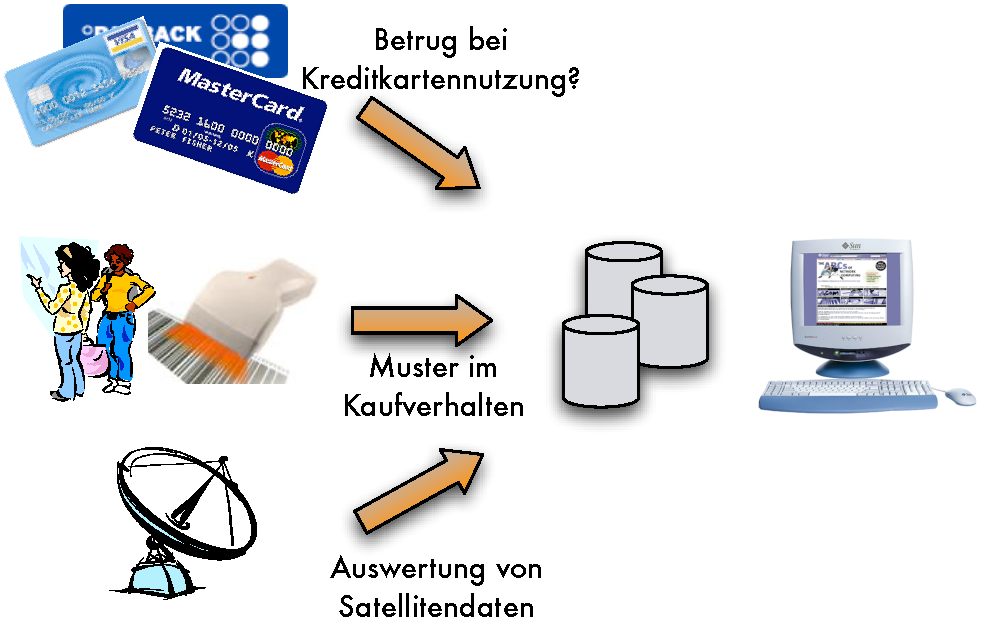
\includegraphics[scale=.5]{fig1/motivation.pdf}
\end{center}


Analyse muss durch "`Vorarbeit"' des Systems unterstützt werden

\end{frame}

%---------------------------------------------------------------------

\begin{frame}
\frametitle{Kommerzieller Bereich}

\begin{minipage}[c]{7cm}
\begin{itemize}
\item Erfassung und Speicherung großer Datenmengen
\begin{itemize}
\item Artikeldaten, Lagerbestände, Warenbewegungen, Lieferantendaten
\item Kaufvorgänge, Kreditkartentransaktionen
\item Nutzerdaten, Kundenbefragungen
\end{itemize}
\item Datenauswertung mit dem Ziel
\begin{itemize}
\item Optimierung der Prozesse
\item Verbesserung des Service
\item Senkung der Kosten
\end{itemize}
\end{itemize}
\end{minipage}\quad
\begin{minipage}[c]{3cm}
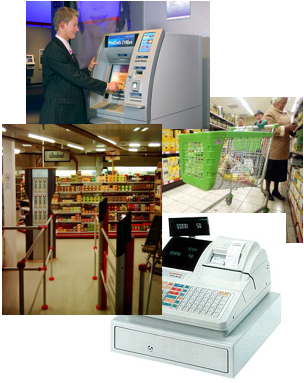
\includegraphics[scale=.3]{fig1/kommerz-anwendung.png}
\end{minipage}

\end{frame}

%---------------------------------------------------------------------

\begin{frame}
\frametitle{Wissenschaftlicher Bereich}

\begin{minipage}[c]{7cm}
\begin{itemize}
\item automatisierte Beobachtung und Erfassung
\begin{itemize}
\item Himmelsteleskope
\item Simulationsmodelle (Wetter, Erdbeben, \dots)
\item Microarrays in der Genforschung
\end{itemize}
\item Produktion riesiger Datenbestände (GB/Stunde)
\begin{itemize}
\item manuelle Aufbereitung und Auswertung kaum mäglich
\end{itemize}
\item Ziele einer Analyse
\begin{itemize}
\item Klassifikation / Segmentierung der Daten
\item Erstellung von Hypothesen
\end{itemize}
\end{itemize}
\end{minipage}\quad
\begin{minipage}[c]{3cm}
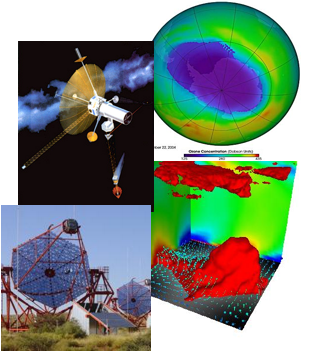
\includegraphics[scale=.3]{fig1/wiss-anwendung.png}
\end{minipage}

\end{frame}

%---------------------------------------------------------------------


\begin{frame}
\frametitle{Analyse großer Datenbestände}

\begin{itemize}
\item Analyse von Daten in Datenbanken (GB \dots PB)
\item "`versteckte"' Informationen: Muster, Abhängigkeiten, \dots
\begin{itemize}
\item manuell nicht identifizierbar
\item aufgrund des Datenvolumens oft überhaupt keine Analyse möglich
\end{itemize}
\end{itemize}


% Abbildung
\begin{center}
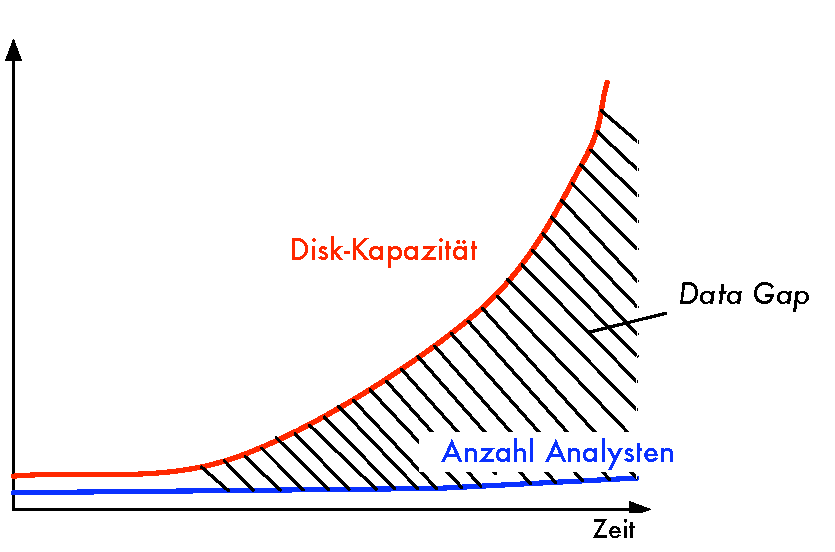
\includegraphics[scale=.45]{fig1/data-gap.pdf}
\end{center}

\end{frame}

%---------------------------------------------------------------------

\begin{frame}
\frametitle{Big Data Analytics}

\begin{itemize}
\item Analyse sehr großer Datenbestände:
\begin{itemize}
\item Fraud Detection bei Kreditkartenunternehmen und
  Finanztransaktionen (Bsp.: Mastercard -- jährlich 8 Mrd. \$ Schaden)
\item  Behavioral Analysis in Suchmaschinen und Sozialen Netzen
\item Genom-und Pharmaforschung
\item \dots
\end{itemize}
\item "`Enabler"': Verfügbarkeit von Speicherkapazität
  (Festplattenproduktion, Cloud), Berechnungskapazität (Serverfarmen), Daten
\item V3: \hl{Volume} (TB $\leadsto$ ZB), \hl{Velocity} (Batch Processing
  $\leadsto$ Realtime/Stream Processing), \hl{Variety} (strukturierte
  $\leadsto$ (semi-)strukturierte Daten)
\end{itemize}

\end{frame}

%---------------------------------------------------------------------

%\begin{frame}
%\frametitle{Data Analytics / ML im Gartner Hype Cycle}
%
%\begin{center}
%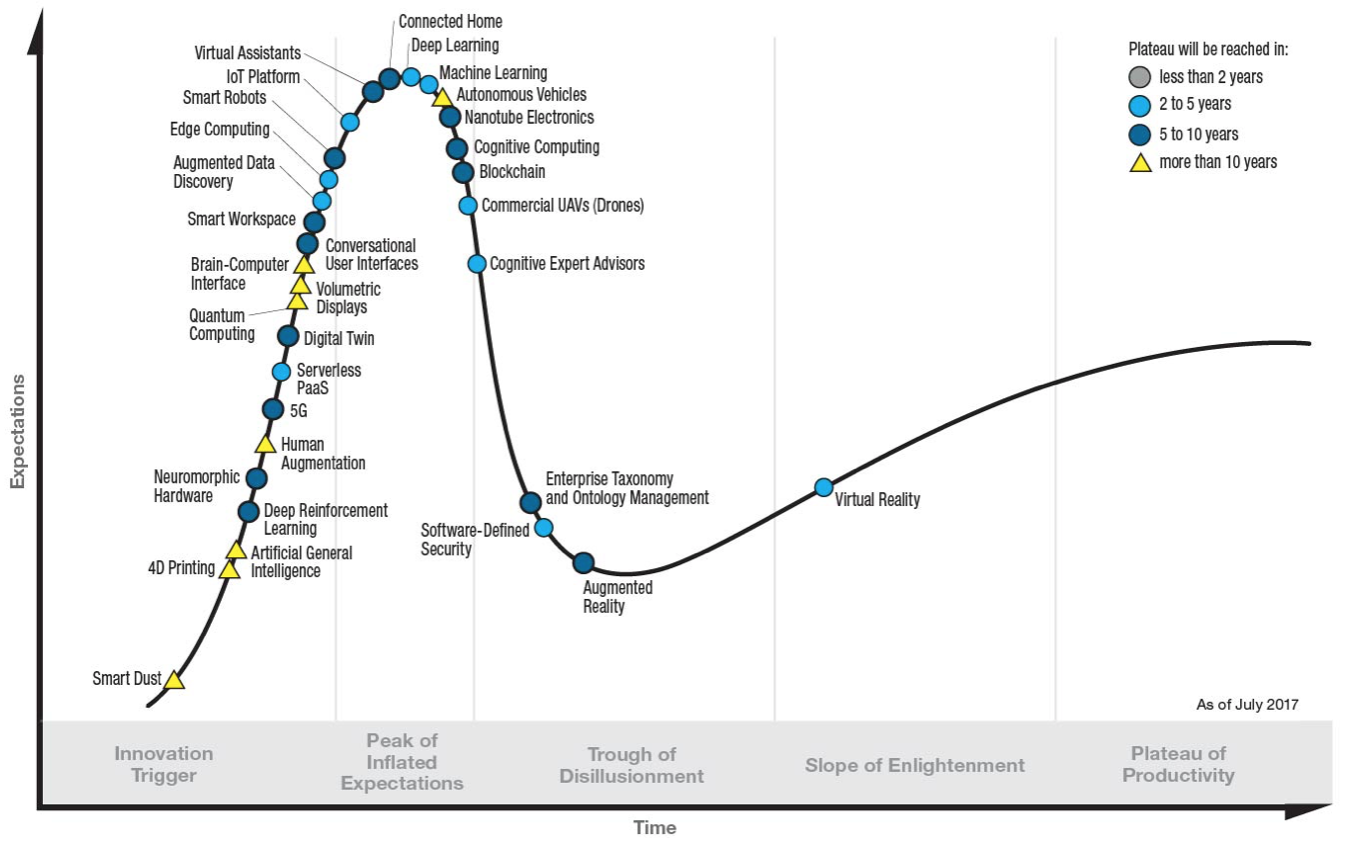
\includegraphics[scale=.45]{fig1/gartner_hype_cycle_2017.png}
%\end{center}
%
%\footnotesize{Quelle: Gartner}
%\end{frame}

%%%%%%%%%%%%%%%%%%%%%%%%%%%%%%%%%%%%%%%%%%%%%%%%%%%%%%%%%%%%%%%%%%%%%%

\section{Begriff Data Science}


\begin{frame}
  \frametitle{Data Science}

  \begin{block}{Data Science}
  interdisziplinäres Wissenschaftsfeld, welches wissenschaftlich fundierte Methoden, Prozesse, Algorithmen und Systeme zur Extraktion von Erkenntnissen, Mustern und Schlüssen sowohl aus strukturierten als auch unstrukturierten Daten ermöglicht (Wikipedia)
  \end{block}

  \begin{itemize}
  \item The key word in "`Data Science"' is not Data, it is Science (Jeff Lesk 2013 @ \url{https://simplystatistics.org/})
  \begin{itemize}
  \item Data Mining als Teilschritt -- Data Science als Prozess
  \item Data Mining/ML-Methoden können in verschiedenen Teilschritten zum Einsatz kommen
  \end{itemize}
  \end{itemize}
  \end{frame}

  %---------------------------------------------------------------------

  \begin{frame}
    \frametitle{Data Science: Einflussgebiete}

    \begin{center}
      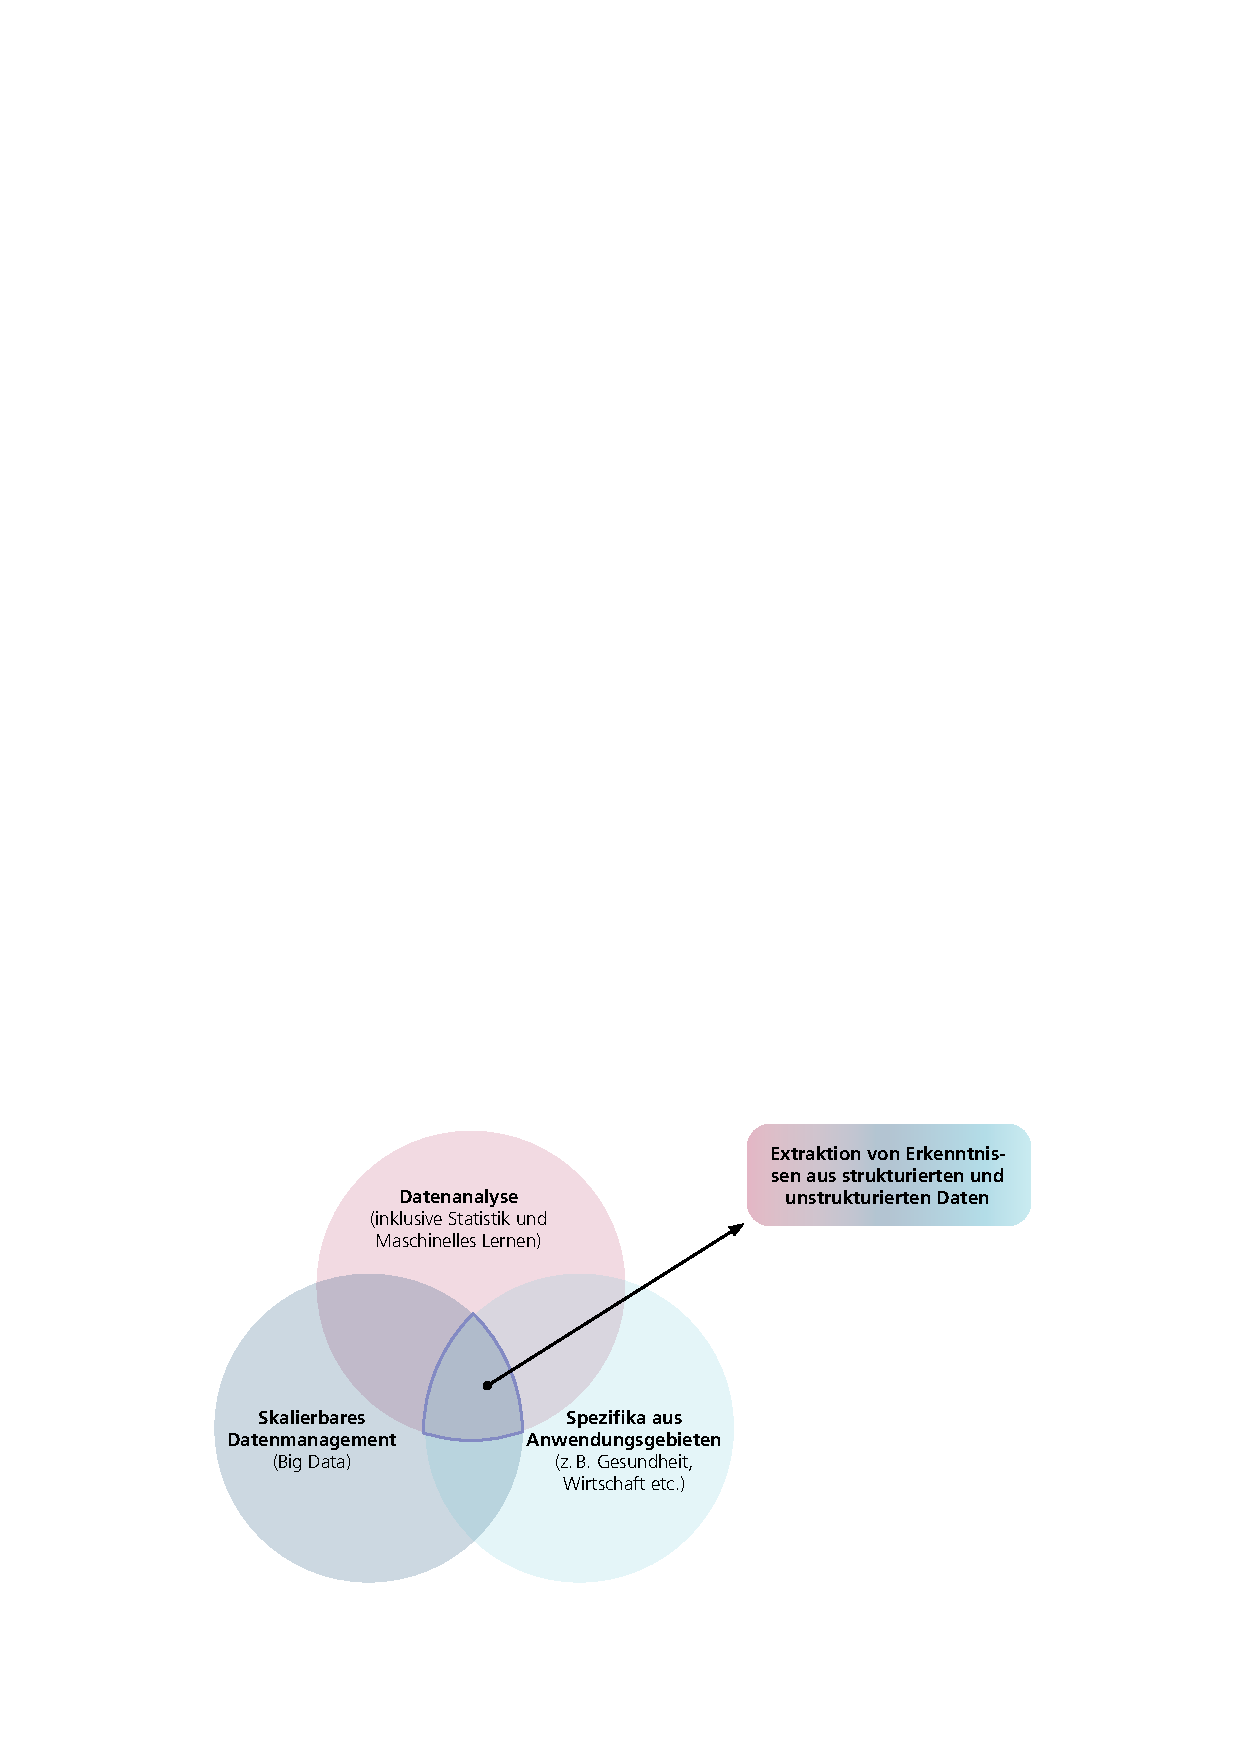
\includegraphics[scale=.7]{fig1/ds-einfluss.pdf}
      \end{center}

  \tiny{Keim, Sattler: Von Daten zu KI --Intelligentes Datenmanagement als Basis für Data Science und den Einsatz Lernender Systeme, Whitepaper Plattform Lernende Systeme, München 2020}
  \end{frame}

  %---------------------------------------------------------------------

\section{Anwendungsbeispiele}

\begin{frame}
  \frametitle{Anwendungsbeispiele}

  \begin{itemize}
\item \hl{Betrugsaufklärung}: Betrugserkennung u.a. bei Banken und Kreditkartenunternehmen durch Analyse der Transaktionsdaten
\item \hl{Medizin}: Systeme zur Unterstützung von Medizinern bei der Diagnose etwa durch Analyse von Röntgenbildern oder Hautbildern zur Krebserkennung
\item \hl{Physik}: Forschung im Bereich der Hochenergiephysik wie das IceCube-Projekt zum Nachweis von Neutrino-Ereignissen oder Arbeiten am LHC des CERN zur Erforschung der Natur der Elementarteilchen und ihrer Wechselwirkungen

\end{itemize}
\end{frame}

%---------------------------------------------------------------------

\begin{frame}
  \frametitle{Anwendungsbeispiele /2}

  \begin{itemize}
    \item \hl{Autonomes Fahren}: zur Klassifikation und Erkennung von Verkehrssituationen anhand der Sensordaten
\item \hl{Sprachassistenten und Übersetzungsdienste}: Erkennung und Übersetzung natürlicher Sprache durch das Training mit großen Datenmengen
\item \hl{Vorausschauende Wartung}: Zustandsüberwachung und vorausschauende Wartung von Produktionsmitteln mit Hilfe von Sensordaten und ML
\item \hl{Werbemarkt}: Modellierung und Vorhersage von Nutzerverhalten

  \end{itemize}
  \end{frame}

%---------------------------------------------------------------------

\section{Datenschutz und Privacy}

\begin{frame}
\frametitle{Datenschutzaspekte}

\begin{itemize}
\item Gefahren des Missbrauchs der Data-Mining-Techniken
\item z.B. wenn personenbezogene Daten ohne Kenntnis der
  betroffenen Person gesammelt und analysiert werden
\item Aspekt des Datenschutzes (Privacy) im Zusammenhang mit Data Mining
\item Beispiele
\begin{itemize}
\item Edward-Snowden-Affäre
\item Wahlkampfmanipulation: Cambridge Analytica
\item Überwachung: Palantir Technologies
\end{itemize}
\end{itemize}

\end{frame}

%---------------------------------------------------------------------

\begin{frame}
\frametitle{Datenschutzaspekte:  Aufdecken von Identitäten}

\begin{itemize}
\item Data Broker Report, FTC Mai 2014
\begin{itemize}
\item Beispiel Acxiom: umfassende Daten von über 700 Mill. Kunden weltweit,
bis zu 1.500 Datenpunkte pro Kunde!
\item Dienste: Marketing, Risikobewertung (Kreditwürdigkeit, Identitäts-/ Missbrauchserkennung), Personensuche
\item Datensammlung aus verschiedensten Quellen (inkl. Offline-Daten) ohne Wissen der Kunden, fehlende Transparenz
\item falsche Risikobewertung, Datenmissbrauch
\end{itemize}
\item Beispiel Target: Erkennung der Schwangerschaft einer Kundin anhand der gekauften Artikel
\item Predictive Policing, Bias
\end{itemize}
\end{frame}

%---------------------------------------------------------------------

\begin{frame}
  \frametitle{Datenschutzaspekte: Persönlichkeitsprofile}

\begin{itemize}
\item Persönlichkeitsprofile aus Facebook-Daten: OCEAN-Modell
\item Offenheit für Erfahrungen (Aufgeschlossenheit)
\item Gewissenhaftigkeit (Perfektionismus)
\item Geselligkeit
\item Verträglichkeit (Rücksichtnahme, Kooperationsbereitschaft, Empathie)
\item Verletzlichkeit
\end{itemize}

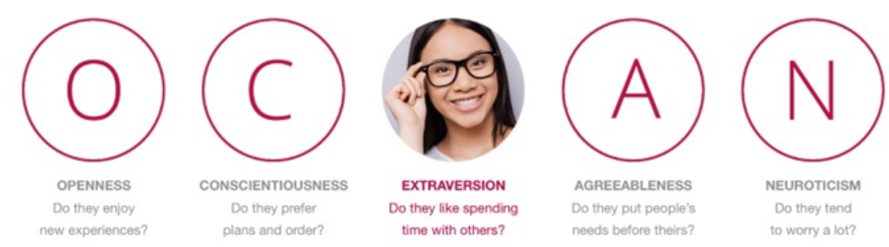
\includegraphics[scale=.7]{fig1/ocean.png}
\end{frame}

%---------------------------------------------------------------------

\begin{frame}
  \frametitle{Datenschutzaspekte: Persönlichkeitsprofile}


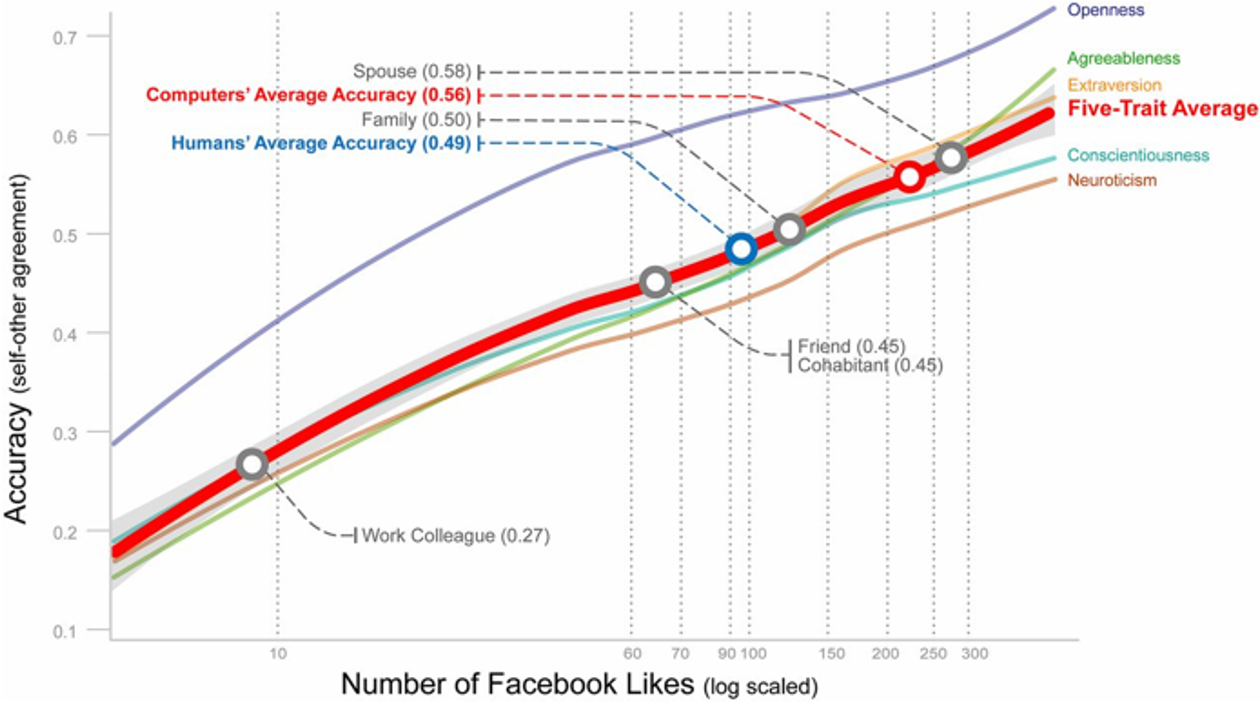
\includegraphics[scale=.5]{fig1/ocean-diagramm.png}

\footnotesize{Youyou, Kosinski, Stillwell Computer-based personality judgments are more accurate than those made by humans, PNAS 2015
}
\end{frame}

%---------------------------------------------------------------------

\begin{frame}
\frametitle{Zusammenfassung}

\begin{itemize}
\item Begriff \hl{Data Science}
\item \hl{Anwendungsbeispiele}
\begin{itemize}
\item Auswertung empirisch erfasster Daten
\item Analyse betriebswirtschaftlicher Daten, wissenschaftlicher
  Daten, Netzwerkdaten (Intrusion Detection, Web Mining, Web Log
  Mining), \dots
\item aber auch Textanalyse (Textklassifikation), Bildanalyse
  (Clustering von Bildern), \dots
\end{itemize}
\item \hl{Datenschutz}
\begin{itemize}
\item wichtiger Aspekt bei der Analyse personenbezogener Daten
\end{itemize}
\end{itemize}

\end{frame}

%---------------------------------------------------------------------

%%% Local Variables:
%%% mode: latex
%%% TeX-master: "main"
%%% End:
